\documentclass[10pt]{article}
\usepackage[margin=2cm]{geometry}
\usepackage{newtxtext,newtxmath}
\usepackage{booktabs,array,threeparttable,url,algorithm,algorithmic,graphicx}
\usepackage[capitalise]{cleveref}
\renewcommand{\thetable}{S\arabic{table}}
\renewcommand{\thefigure}{S\arabic{figure}}
\renewcommand{\thesection}{S\arabic{section}}
\title{Supplementary Material:\\Auditing SHAP Explanations Against Known Failure Mechanisms in Predictive Maintenance}
\author{Koshik Debanath, Prakrit Uprety, and Peiyu Li}
\date{}
\begin{document}
\maketitle

Numerical tables are generated from stored result files by the accompanying scripts. The immutable computational snapshot is \texttt{tuai-computation-5b97414ab7ef.zip}, with full SHA-256 recorded in its accompanying checksum file and per-file hashes in \texttt{SNAPSHOT\_MANIFEST.json}. Source repository: \url{https://github.com/kowshik24/shap-mechanism-audit}. This local snapshot does not establish public release availability; stage numbers refer to \texttt{experiments/NN\_*.py}. Holm-adjusted $p$-values throughout.

\section{Implementation}

\paragraph{Classifiers} \Cref{tab:config} lists the settings of the seven benchmark classifiers and \cref{tab:models} their failure-class test performance (scikit-learn 1.9.1, XGBoost 3.4.1, PyTorch 2.14.0; seed 42). Precision and recall intervals are Clopper--Pearson, the others 5{,}000 stratified bootstrap resamples. Five-fold cross-validation of tuned XGBoost at threshold 0.5 gives failure-class F1 $0.822\pm0.013$; its Brier score is 0.0090 (0.033 for a base-rate predictor) and its expected calibration error 0.008.

\begin{table}[htbp]
\centering
\caption{Classifier settings.}
\label{tab:config}
\small
\begin{tabular}{@{}lp{5.6cm}@{}}
\toprule
Model & Settings \\
\midrule
Logistic regression & max.\ 1000 iterations \\
SVM & radial basis function (RBF) kernel, probability outputs \\
$k$-NN & $k = 7$ \\
Decision tree & max.\ depth 10 \\
Random forest & 300 trees, max.\ depth 12 \\
XGBoost & 300 trees, max.\ depth 6, learning rate 0.1 \\
XGBoost (tuned) & 200 trees, max.\ depth 8, learning rate 0.1, subsample 0.8, column sample 0.8, min.\ child weight 1, $\gamma = 0$ \\
MLP & 64 and 32 hidden units, ReLU, batch norm, dropout 0.3/0.2; Adam (learning rate $10^{-3}$, weight decay $10^{-5}$), binary cross-entropy, batch 64, 40 epochs \\
\bottomrule
\end{tabular}

\end{table}

\begin{table}[htbp]
\centering
\caption{Failure-class test performance, sorted by F1; parentheses: 95\% bootstrap interval for F1.}
\label{tab:models}
\small
\begin{tabular}{@{}lrrlr@{}}
\toprule
Model & Prec. & Rec. & F1 (95\% CI) & ROC-AUC \\
\midrule
XGBoost (tuned) & \textbf{1.00} & 0.79 & \textbf{0.89} (0.79--0.95) & 0.988 \\
XGBoost & 0.86 & 0.88 & 0.87 (0.78--0.94) & 0.988 \\
Random forest & 0.79 & 0.88 & 0.83 (0.74--0.92) & \textbf{0.989} \\
MLP & 0.65 & \textbf{0.91} & 0.76 (0.67--0.84) & 0.988 \\
Decision tree & 0.68 & 0.82 & 0.75 (0.64--0.84) & 0.927 \\
SVM & 0.42 & 0.88 & 0.57 (0.48--0.65) & 0.976 \\
k-NN & 0.43 & 0.79 & 0.56 (0.46--0.65) & 0.877 \\
Logistic regression & 0.24 & 0.85 & 0.37 (0.31--0.43) & 0.943 \\
\bottomrule
\end{tabular}

\end{table}

\paragraph{Explainers and variants} Interventional TreeSHAP draws 100, 500, or 1{,}000 background observations per fold from the original (not oversampled) training data with three background seeds, or, for TWF, 100 observations only from non-failures, only from failures, or from the oversampled training set. The pairwise reference is the nearest normal-operation training observation of each explained observation. The MLP (64 and 32 hidden units) is explained on its logit by KernelSHAP (25 background observations, 1{,}000 coalitions; exact with 100 or 500 background observations and all 4{,}096 coalitions; or 25 weighted k-means centres), Integrated Gradients (1{,}024 steps from the mean of 100 training observations, completeness within 5\%), DeepSHAP (100 background observations), and SmoothGrad (50 samples, noise s.d.\ 0.15 in standardized units, times the input's difference from the same mean). LIME explains the failure probability of the XGBoost pipeline with 1{,}000 perturbations per observation and the fold's training data. Grouped TreeSHAP sums signed path-dependent SHAP over four groups (wear: tool wear, overstrain, its ratio; thermal: both temperatures, their difference; load: torque, speed, power; type), and the conditional group Shapley values evaluate all 16 coalitions with Gaussian kernel weights over 2{,}000 training observations of the fold (bandwidth 0.3 in standardized units). Every variant uses a null of the same pipeline.

\section{Detailed Evaluation Protocol}
\label{sec:protocol}
The main paper retains the audit definitions and the design choices needed to interpret its results. The following protocol supplies implementation and sampling details.

\paragraph{AI4I feature construction} Several rules combine sensor readings, so we construct mechanical power
$P=\tau(2\pi n/60)$, temperature difference
$\Delta T=T_{\mathrm{process}}-T_{\mathrm{air}}$,
overstrain $O=w\tau$, and overstrain ratio $Q=O/L(t)$,
where $\tau$, $n$, and $w$ denote torque, rotational speed,
and tool wear, and the type-specific limit $L(t)$
is 11{,}000, 12{,}000, or 13{,}000 for types
\texttt{L}, \texttt{M}, and \texttt{H}. The set $E_m$ contains every input that appears in a rule's condition, either directly or as the quantity in which the condition is written. The OSF condition compares overstrain with a type-specific limit, so $E_{\mathrm{OSF}}$ contains $Q$, which expresses this comparison, but not the type indicators, which carry no OSF information on their own. The engineered features encode the documented benchmark rules and use no labels. AI4I therefore tests whether attributions follow known rules, and it cannot show that a model discovers unknown physical relationships. We also repeat the audit on the original features only; the main paper reports the resulting verdicts.


\paragraph{AI4I label handling} Twenty-four observations have overlapping mechanism flags, nine released-label failures have none, and 18 of the 19 RNF observations are labeled non-failures. The primary audit uses the released labels and every mechanism-positive row. Sensitivity checks use single-flag rows, remove unflagged failures, or rebuild the label as the OR of the mechanism flags. RNF has no expected feature set and is descriptive only.

\paragraph{Model selection and evaluation} We split the data into stratified training, validation, and test sets (70/20/10). On these splits we select the preprocessing (scaling and one-hot encoding fitted on the training set), the oversampler (Borderline-SMOTE, chosen over SMOTE and ADASYN by the validation F1 of a default XGBoost), the XGBoost hyperparameters (40-iteration randomized search with five-fold cross-validation on the training set, oversampling inside each fold), and the decision threshold (validation F1). The reserved test split provides predictive-performance estimates in the main paper; the attribution audit separately cross-fits over the full dataset. Classifier settings and performance are listed in \cref{tab:config,tab:models}.

For the audit, these choices are fixed and the full pipeline (preprocessing, oversampling, training) is refitted by five-fold stratified cross-fitting over all 10{,}000 observations. Each fold's model explains only its held-out fifth, so no observation is explained by a model that was trained on it. Model selection is not nested within the audit folds, and the re-tuned null repeats the selection on every permutation to assess sensitivity to this choice; it does not make the original-label audit nested. Attributions do not depend on the threshold.


\paragraph{Controlled perturbations and scaling} We run three groups of experiments on AI4I. The audit variants change one part of the primary configuration at a time, such as the data and expected sets, the imbalance treatment, the attribution method and reference, the model, or the null, and each variant is compared with its own null (full tests in \cref{tab:full}). For the planted shortcut we add a sensor $s_i=z_{i,\mathrm{HDF}}+\epsilon_i$, $\epsilon_i\sim\mathcal{N}(0,\sigma^2)$, a noisy copy of the HDF flag with no physical role, excluded from $E_{\mathrm{HDF}}$, and decrease $\sigma$ from 2 to 0.1 ($K=500$). For the scaling study we generate data from the documented AI4I process with $n\in\{10^4,3\cdot10^4,10^5,3\cdot10^5\}$ (three generation seeds, one at $3\cdot10^5$), without a sensor and with $\sigma\in\{0.35,0.25\}$ ($K=200$).

\paragraph{CWRU bearings (laboratory)} We use 36 drive-end vibration recordings (12~kHz) with seeded faults at three locations (inner race, ball, outer race), three sizes, and four motor loads. A random forest (100 trees, depth 8) classifies the fault location from 19 features per 4{,}096-sample window. $S_m$ contains the windows of fault $m$ and the comparison group contains the windows of the other faults. Each window is explained through the output of its own class, so $D_m$ compares how strongly fault-$m$ windows use the defect frequencies of $m$ with how strongly the other windows use them for their own diagnosis. $E_m$ holds the spectral power within $\pm0.15$ shaft orders of the defect frequency and its second harmonic in the raw and envelope (2--5~kHz band-pass) spectra (defect orders 5.42, 4.71, and 3.58 for the SKF~6205 bearing). Four-fold stratified group cross-fitting holds out whole recordings, and the null permutes fault labels across recordings ($K=1{,}000$). A gain shortcut scales each recording's amplitude by a fault-dependent factor (0.25, 1, 4), which changes only the log-RMS feature.

\paragraph{Tennessee Eastman process (simulated)} We use 400 runs of the DTU set, 200 each with a step in the reactor (IDV4) or condenser (IDV5) cooling-water inlet temperature at 30~h, and take 16 samples of all 53 variables before (10--25~h) and 16 after (40--95~h) the fault. The label is fault activity, $S_m$ contains the fault-active samples of fault $m$, the comparison group contains those of the other fault, and $E_m$ holds the three variables of the disturbed loop. XGBoost (300 trees, depth 6) uses five-fold stratified group cross-fitting over whole runs. The null permutes labels within each run, preserving its sensor trajectory and counts of 16 normal and 16 faulty samples ($K=200$). It breaks the time--label association and does not preserve temporal dependence in the labels, so we also use a second null that rotates each run's time-ordered labels by a random offset and keeps the fault-active samples in one contiguous block. Neither reference establishes exchangeability of the temporal labels. A temporal variant adds each variable's 30-minute mean and change and sums attribution per variable. A second variant classifies 30-minute sequences with an LSTM (32 units) and explains them with Integrated Gradients summed over time.


\paragraph{Aggregation and uncertainty} For example, on the 95 PWF observations, power, torque, and speed have mean $|\phi|$ of 4.96, 1.93, and 1.33, out of 11.82 over all twelve inputs, so $R_{\mathrm{PWF}}\approx0.70$. We use absolute values so that positive and negative contributions do not cancel and so that a feature pushing a prediction away from failure still counts as used; the direction of attribution is checked separately. A large $C_m$ can come from a shortcut, from a trigger that is missing in $E_m$, or from a downstream effect of the mechanism. A flag therefore names a feature that should be inspected, and it does not by itself identify the cause.

 Per-observation normalization before averaging changes the observed primary $R_m$ and $D_m$ by at most 0.02. We report $z=(T-\bar T_0)/s_0$ and 95\% percentile bootstrap intervals for $R_m$ and $D_m$ from 5,000 within-group resamples, conditional on the fitted models. The primary verdicts are also unchanged when Holm correction is applied over all twelve tests rather than separately within each four-mechanism statistic family; requiring both alignment tests to reject is an intersection--union decision.

\section{Primary audit pseudocode}

The following algorithm describes the five-fold AI4I audit with fixed hyperparameters. CWRU instead uses four recording-group folds and recording-label permutations; TEP uses five run-group folds and within-run label permutations, as specified in the paper. Model selection is not nested in the AI4I audit.

\begin{algorithm}[H]
\caption{Mechanism-level attribution audit}
\label{alg:audit}
\small
\begin{algorithmic}[1]
\REQUIRE data $(x_i,y_i,z_i)$, expected sets $E_m$, pipeline $\mathcal{P}$, explainer $\phi$, $K$, $\alpha$
\STATE $A\leftarrow$ held-out $|\phi|$ from five-fold cross-fitting of $\mathcal{P}$ on $(x,y)$
\STATE compute $R_m$, $D_m$, $C_m$ from $A$ for every mechanism $m$ (Eqs.~(2)--(4) of the paper)
\FOR{$k=1$ \TO $K$}
\STATE $y^{(k)}\leftarrow$ random permutation of $y$; keep $x$ and $z$
\STATE $A^{(k)}\leftarrow$ held-out $|\phi|$ from cross-fitting $\mathcal{P}$ on $(x,y^{(k)})$
\STATE compute $R_m^{(k)}$, $D_m^{(k)}$, $C_m^{(k)}$ from $A^{(k)}$
\ENDFOR
\STATE $p$-values by Eq.~(5) of the paper; Holm correction over mechanisms for each statistic
\FOR{each mechanism $m$}
\IF{$p_{C,m}<\alpha$}
\STATE flagged; report the feature with the largest excess
\ELSIF{$p_{R,m}<\alpha$ and $p_{D,m}<\alpha$}
\STATE aligned
\ELSE
\STATE not aligned
\ENDIF
\ENDFOR
\ENSURE verdicts, flagged features and excesses, effect sizes $z$, bootstrap intervals
\end{algorithmic}
\end{algorithm}

\section{Reporting checklist}

The following steps summarize the audit configuration we recommend fixing and reporting.
\begin{enumerate}
\item \textbf{Mechanism map.} Fix $E_m$ from rules or physics before the audit. State which inputs are engineered from a documented rule, and repeat the audit on the original inputs to show how much the engineered features contribute.
\item \textbf{Attribution.} State the explainer, the explained output (logit or probability), and the reference distribution. Match the reference to the question. To ask which features make an observation look abnormal, measure against normal operation (interventional background of non-failures or a nearest normal observation). To ask how the model uses its training data, path-dependent TreeSHAP or a background drawn from the training data is appropriate, but with oversampling it treats ordinary values as evidence against failure (TWF in the paper). Neither answers counterfactual or root-cause questions. When the references disagree, report both.
\item \textbf{Held-out explanations.} Explain each observation with a model that did not train on it; hold out whole recordings or runs when observations within them are dependent.
\item \textbf{Null.} Refit the full pipeline (preprocessing, resampling, training, explanation) on shuffled labels. Permute within groups, and shift labels in time when they are temporally dependent. With $M$ mechanisms, Holm correction needs $K\geq M/\alpha$ before any test can pass (80 for $M=4$); for a Monte Carlo standard error $e$ of a raw $p$-value near $\alpha$, choose $K\geq\alpha(1-\alpha)/e^2$ (\cref{sec:k}). In practice use $K\geq200$, and $K\geq500$ when an adjusted $p$ lies near $\alpha$.
\item \textbf{Verdicts.} Apply Holm correction across mechanisms for each statistic and report $R_m$, $D_m$, and $C_m$ with their null means, $z$, and bootstrap intervals, not only the verdict.
\item \textbf{Flags.} Report the flagged feature and its excess. The 0.05 excess cutoff explored in this study was selected post hoc, not validated; report excess sizes and inspect each flag for a missing trigger, a downstream effect, or a shortcut.
\item \textbf{Stability.} Repeat the audit over seeds, background samples, and at least one alternative explainer or reference, and report verdicts that change.
\end{enumerate}

\clearpage
\section{Full audit $p$-values}

\Cref{tab:full} gives the Holm-adjusted $p$-values for all variants, including the selected variants in Table~III of the paper. The main table omits background-size, neighbour-count, and other implementation variants to keep the main comparisons readable.

\begin{table}[H]
\centering
\begin{threeparttable}
\caption{Holm-adjusted $p$-values of the $R$, $D$, and $C$ tests for every audit variant. $^{\times}$: non-significant alignment test; $^{\dagger}$: significant outside-set test; minimum attainable adjusted $p$: $4/(K+1)$.}
\label{tab:full}
\scriptsize
\setlength{\tabcolsep}{3pt}
\begin{tabular}{@{}lrrrrrrrrrrrrr@{}}
\toprule
& & \multicolumn{3}{c}{TWF} & \multicolumn{3}{c}{HDF} & \multicolumn{3}{c}{PWF} & \multicolumn{3}{c}{OSF} \\
\cmidrule(lr){3-5}\cmidrule(lr){6-8}\cmidrule(lr){9-11}\cmidrule(lr){12-14}
Variant & $K$ & $R$ & $D$ & $C$ & $R$ & $D$ & $C$ & $R$ & $D$ & $C$ & $R$ & $D$ & $C$ \\
\midrule
Primary, seed 42 & 1000 & 0.201$^{\times}$ & 0.077$^{\times}$ & 1.000 & 0.004 & 0.004 & 1.000 & 0.004 & 0.004 & 1.000 & 0.004 & 0.004 & 1.000 \\
\quad single-mechanism rows & 1000 & 0.187$^{\times}$ & 0.076$^{\times}$ & 1.000 & 0.004 & 0.004 & 1.000 & 0.004 & 0.004 & 1.000 & 0.004 & 0.004 & 1.000 \\
\quad null re-tuned per permutation & 500 & 0.447$^{\times}$ & 0.359$^{\times}$ & 1.000 & 0.018 & 0.008 & 1.000 & 0.008 & 0.008 & 1.000 & 0.032 & 0.008 & 1.000 \\
\quad positive part of SHAP & 200 & 0.020 & 0.020 & 1.000 & 0.020 & 0.020 & 1.000 & 0.020 & 0.020 & 1.000 & 0.020 & 0.020 & 1.000 \\
Seeds 1--4 (largest $p$) & 200 & 0.269$^{\times}$ & 0.129$^{\times}$ & 1.000 & 0.020 & 0.020 & 1.000 & 0.020 & 0.020 & 1.000 & 0.020 & 0.020 & 1.000 \\
Raw features only & 1000 & 0.345$^{\times}$ & 0.616$^{\times}$ & 1.000 & 0.190$^{\times}$ & 0.004 & 1.000 & 0.004 & 0.004 & 1.000 & 0.004 & 0.048 & 1.000 \\
In-sample SHAP & 1000 & 0.004 & 0.004 & 1.000 & 0.004 & 0.004 & 1.000 & 0.004 & 0.004 & 1.000 & 0.004 & 0.004 & 1.000 \\
\addlinespace
Unflagged failures removed & 200 & 0.179$^{\times}$ & 0.075$^{\times}$ & 1.000 & 0.020 & 0.020 & 1.000 & 0.020 & 0.020 & 1.000 & 0.020 & 0.020 & 1.000 \\
Label = OR of flags & 200 & 0.308$^{\times}$ & 0.144$^{\times}$ & 1.000 & 0.020 & 0.020 & 1.000 & 0.020 & 0.020 & 1.000 & 0.020 & 0.020 & 1.000 \\
Class weights, no oversampling & 200 & 0.085$^{\times}$ & 0.020 & 1.000 & 0.020 & 0.020 & 1.000 & 0.020 & 0.020 & 1.000 & 0.020 & 0.020 & 1.000 \\
Focal loss, no oversampling & 200 & 0.020 & 0.020 & 1.000 & 0.020 & 0.020 & 1.000 & 0.020 & 0.020 & 1.000 & 0.020 & 0.020 & 1.000 \\
Borderline-SMOTE, 3 neighbours & 200 & 0.184$^{\times}$ & 0.0498 & 1.000 & 0.020 & 0.020 & 1.000 & 0.020 & 0.020 & 1.000 & 0.020 & 0.020 & 1.000 \\
Borderline-SMOTE, 10 neighbours & 200 & 0.269$^{\times}$ & 0.149$^{\times}$ & 1.000 & 0.020 & 0.020 & 1.000 & 0.020 & 0.020 & 1.000 & 0.020 & 0.020 & 1.000 \\
SMOTE & 200 & 0.169$^{\times}$ & 0.085$^{\times}$ & 1.000 & 0.109$^{\times}$ & 0.020 & 1.000 & 0.020 & 0.020 & 1.000 & 0.020 & 0.020 & 1.000 \\
ADASYN & 200 & 0.159$^{\times}$ & 0.090$^{\times}$ & 0.955 & 0.109$^{\times}$ & 0.020 & 1.000 & 0.020 & 0.020 & 1.000 & 0.020 & 0.020 & 1.000 \\
$E_m$ without derived features & 200 & 0.468$^{\times}$ & 0.209$^{\times}$ & 0.478 & 0.040 & 0.020 & 0.020$^{\dagger}$ & 0.179$^{\times}$ & 1.000$^{\times}$ & 0.020$^{\dagger}$ & 0.776$^{\times}$ & 1.000$^{\times}$ & 0.020$^{\dagger}$ \\
$E_m$ without top trigger & 200 & 0.701$^{\times}$ & 0.209$^{\times}$ & 0.478 & 0.995$^{\times}$ & 0.020 & 0.020$^{\dagger}$ & 0.239$^{\times}$ & 0.935$^{\times}$ & 0.020$^{\dagger}$ & 0.995$^{\times}$ & 0.657$^{\times}$ & 0.020$^{\dagger}$ \\
\addlinespace
Interventional, background 100 & 200 & 0.020 & 0.020 & 1.000 & 0.020 & 0.020 & 1.000 & 0.020 & 0.020 & 1.000 & 0.020 & 0.020 & 1.000 \\
\quad failure-only background & 200 & 0.995$^{\times}$ & 0.945$^{\times}$ & 0.020$^{\dagger}$ & 0.826$^{\times}$ & 0.149$^{\times}$ & 1.000 & 0.045 & 0.090$^{\times}$ & 1.000 & 0.040 & 0.020 & 1.000 \\
\quad non-failure background & 200 & 0.020 & 0.020 & 1.000 & 0.020 & 0.020 & 1.000 & 0.020 & 0.020 & 1.000 & 0.020 & 0.020 & 1.000 \\
\quad oversampled background & 200 & 0.045 & 0.020 & 0.896 & 0.020 & 0.020 & 1.000 & 0.020 & 0.020 & 1.000 & 0.020 & 0.020 & 1.000 \\
Pairwise (nearest normal reference) & 200 & 0.020 & 0.020 & 0.498 & 0.020 & 0.020 & 1.000 & 0.020 & 0.020 & 1.000 & 0.020 & 0.020 & 1.000 \\
Random forest & 200 & 0.617$^{\times}$ & 0.398$^{\times}$ & 1.000 & 0.020 & 0.020 & 1.000 & 0.020 & 0.020 & 1.000 & 0.040 & 0.020 & 1.000 \\
Grouped TreeSHAP (4 groups) & 200 & 0.816$^{\times}$ & 1.000$^{\times}$ & 1.000 & 0.020 & 0.020 & 1.000 & 0.020 & 0.020 & 1.000 & 0.020 & 0.030 & 1.000 \\
Conditional group Shapley & 200 & 0.020 & 0.020 & 1.000 & 0.020 & 0.040 & 0.517 & 0.020 & 0.020 & 1.000 & 0.020 & 0.040 & 1.000 \\
LIME & 200 & 0.040 & 0.020 & 1.000 & 0.020 & 0.020 & 1.000 & 0.020 & 0.159$^{\times}$ & 1.000 & 0.040 & 0.020 & 0.597 \\
\addlinespace
MLP, KernelSHAP & 200 & 0.975$^{\times}$ & 0.831$^{\times}$ & 0.975 & 0.388$^{\times}$ & 0.189$^{\times}$ & 1.000 & 0.358$^{\times}$ & 0.020 & 1.000 & 0.358$^{\times}$ & 0.075$^{\times}$ & 1.000 \\
\quad exact, background 100 & 200 & 1.000$^{\times}$ & 0.915$^{\times}$ & 0.756 & 0.557$^{\times}$ & 0.219$^{\times}$ & 0.965 & 0.557$^{\times}$ & 0.020 & 0.965 & 0.557$^{\times}$ & 0.149$^{\times}$ & 0.851 \\
\quad exact, background 500 & 100 & 0.990$^{\times}$ & 0.881$^{\times}$ & 0.792 & 0.683$^{\times}$ & 0.337$^{\times}$ & 1.000 & 0.683$^{\times}$ & 0.040 & 1.000 & 0.277$^{\times}$ & 0.089$^{\times}$ & 1.000 \\
\quad k-means background & 200 & 0.980$^{\times}$ & 0.900$^{\times}$ & 0.637 & 0.547$^{\times}$ & 0.299$^{\times}$ & 1.000 & 0.493$^{\times}$ & 0.045 & 1.000 & 0.080$^{\times}$ & 0.020 & 1.000 \\
MLP, Integrated Gradients & 200 & 0.338$^{\times}$ & 0.100$^{\times}$ & 0.522 & 0.020 & 0.020 & 1.000 & 0.0498 & 0.100$^{\times}$ & 0.478 & 0.030 & 0.020 & 1.000 \\
MLP, DeepSHAP & 200 & 0.920$^{\times}$ & 0.368$^{\times}$ & 0.478 & 0.020 & 0.020 & 1.000 & 0.104$^{\times}$ & 0.045 & 1.000 & 0.129$^{\times}$ & 0.045 & 1.000 \\
MLP, SmoothGrad & 200 & 0.970$^{\times}$ & 0.677$^{\times}$ & 0.040$^{\dagger}$ & 0.020 & 0.020 & 1.000 & 0.0498 & 0.020 & 1.000 & 0.020 & 0.020 & 1.000 \\
\addlinespace
Permuted labels (sanity) & 200 & 1.000$^{\times}$ & 0.731$^{\times}$ & 1.000 & 0.199$^{\times}$ & 0.557$^{\times}$ & 1.000 & 1.000$^{\times}$ & 0.731$^{\times}$ & 1.000 & 1.000$^{\times}$ & 0.731$^{\times}$ & 0.637 \\
\bottomrule
\end{tabular}

\end{threeparttable}
\end{table}

\section{Choice of $K$}
\label{sec:k}

The Monte Carlo standard error of a raw $p$-value near $\alpha=0.05$ is $\sqrt{\alpha(1-\alpha)/K}$: 0.022, 0.015, 0.010, and 0.007 for $K=100$, 200, 500, and 1{,}000. This is the error of a raw $p$-value; the uncertainty of a Holm-adjusted decision also depends on the other mechanisms' $p$-values. Primary verdicts are identical at $K=100$, 200, 500, and 1{,}000, so we recommend $K\geq200$, and $K\geq500$ when an adjusted $p$ lies within 0.03 of $\alpha$. Across 40 mechanism and size combinations of the scaling runs, the null standard deviation of $R_m$ falls only slowly with mechanism size (log--log slope $-0.14$), so the same $K$ serves small and large mechanisms.

\section{Exploratory power approximation}

For the $R$ and $D$ tests of the primary audit we approximate power at the first Holm step, the most demanding one. Assume the null statistic is normal with the observed null mean $\bar{T}_0$ and s.d.\ $s_0$, so that the critical value is $c=\bar{T}_0+z_{1-\alpha/4}s_0$, and that the observed statistic is normal around its value $T$ with the bootstrap s.d.\ $s_b$ (conditional on the fitted models). Power is then $\Phi((T-c)/s_b)$, and the minimum excess over $\bar{T}_0$ detectable with 80\% power is $z_{1-\alpha/4}s_0+z_{0.8}s_b$. The approximation gives power near 1 for HDF, PWF, and OSF and 0.00 ($R$) and 0.02 ($D$) for TWF; the minimum detectable excess is 0.10--0.14. These numbers rest on normality and on a bootstrap that ignores refitting variability, and are exploratory.

\section{Alternative statistics}
\label{sec:alternatives}

\paragraph{Rank-based alignment} $Rk_m$ is the per-observation probability that an expected feature outranks a non-expected one in $|\phi|$, averaged over $S_m$, and $Dk_m$ its difference to other failures (stage 20, $K=200$). On the primary audit they align PWF and OSF, but HDF fails $Rk$ ($p=0.33$). Under both misspecified expected sets of the paper, they align no mechanism. They are therefore not less brittle to an incomplete $E_m$ and are less powerful than $R_m$ and $D_m$.

\paragraph{Outside-set alternatives} (i) A studentized maximum (each feature's excess standardized by its own null mean and s.d.) is less sensitive than $C_m$ in the shortcut sweep: it first flags the sensor at $\sigma=0.20$ ($p=0.032$), versus $\sigma=0.25$ for $C_m$. (ii) A null-referenced score (each outside feature's share on $S_m$ standardized against the null, without other failures) flags TWF in every setting, including the primary audit (on speed or torque, which the model uses for all failures), and misses the sensor at $\sigma=0.25$ ($p=0.39$). (iii) $C_m$ computed on the failure-pushing part of SHAP, $\max(\phi,0)$, does not flag the sensor at any tested strength ($p=0.139$ at $\sigma=0.25$), although it flags the omitted triggers.

\section{Supporting Controls and Diagnostic Results}
\label{sec:diagnostics}
\paragraph{Robustness diagnostics} Table~III of the main paper summarizes selected variants; the supplement reports every variant and all three test results. Other seeds and the restriction to single-mechanism observations change nothing. Across five seeds, $R_m$ varies by at most 0.02 and every mechanism keeps the same three most attributed features; across seven interventional background sizes and seeds, it varies by at most 0.015. Re-tuning the hyperparameters on each of 500 permutations widens the null (the 95th percentile of $R_{\mathrm{OSF}}$ rises from 0.45 to 0.61) and leaves the results unchanged, although the relevant share of OSF moves closer to the threshold ($p=0.032$). Without the engineered features, the excess of $R_m$ over its null mean shrinks by 0.02--0.10 (HDF: from 0.15 to 0.06), PWF and OSF stay aligned, and HDF no longer passes the relevant-share test ($p=0.19$), consistent with difficulty representing the temperature-difference rule using separate temperature inputs. Label corrections change nothing, but the oversampler does matter. With SMOTE or ADASYN, HDF no longer passes the relevant-share test ($p=0.109$), and a focal-loss model trained without oversampling aligns TWF. When we removed the derived features or each mechanism's most attributed trigger from $E_m$, the affected mechanisms were flagged, and each flag named the omitted feature.

\paragraph{Supporting checks} Three further checks, which do not enter the audit decision, look at direction, feature removal, and statistical dependence. On mechanism observations, 97--99\% of the trigger features' attribution pushes toward failure (30--67\% on other failures). Retraining without a mechanism's raw trigger features cuts recall on its observations from 0.94 to 0.23 (HDF), 0.85 to 0.01 (PWF), and 0.95 to 0.23 (OSF). An HSIC check between each input and the held-out prediction ranks a trigger feature first for all four mechanisms (rank correlation with the SHAP shares 0.27--0.90). These checks agree with the aligned results for HDF, PWF, and OSF. For TWF, HSIC ranks tool wear first even though the audit does not align the mechanism, which is consistent with the reference dependence discussed in the main paper.


\paragraph{Tool-wear reference diagnostics} The earlier interpretation emphasized correlation between tool wear and engineered overstrain features. Recomputing Spearman correlation between wear $w$ and the overstrain product $w\tau$ gives 0.92 overall but only 0.13 on TWF observations. Interventional TreeSHAP still aligns TWF with original inputs only, whereas summing path-dependent SHAP over feature groups does not. A non-failure background aligns TWF, and a failure-only background removes that alignment and produces an outside-set flag. The background comparisons therefore support a reference-distribution explanation rather than treating overall correlation as sufficient. Conditional Shapley results concern the specified feature groups and kernel bandwidths, not unrestricted conditional SHAP. These diagnostics qualify the interpretation without identifying a unique causal explanation for the verdict change.

\paragraph{Single-sensor shortcut sweep} The single-sensor sweep shows two distinct audit outcomes. Weak shortcuts ($\sigma\geq0.35$, at most 13\% of HDF attribution) leave HDF aligned. A moderate shortcut ($\sigma=0.30$, 21\%) removes the alignment because the relevant-share test fails, but no feature is flagged. Stronger shortcuts ($\sigma\leq0.25$, at least 35\%) are flagged by the outside-set test, which names the sensor. Test F1 stays between 0.84 and 0.92 in all settings, and PWF and OSF remain aligned. These strengths apply to this particular sensor and sample size. Two alternative outside-set statistics, one standardized against the null alone and one computed on failure-pushing attribution, did not flag the sensor earlier (see \cref{sec:alternatives}). When the planted signal is split over three sensors with independent noise, the model spreads attribution over them. At $\sigma=0.35$ they receive 38\% of HDF attribution together, more than the single sensor flagged at $\sigma=0.25$, but at most 14\% each. HDF is then not aligned, yet no feature is flagged until $\sigma=0.25$ (54\% together). Because $C_m$ takes the maximum over single features, a shortcut spread over several inputs is harder to name.


\paragraph{Sample-size effects and computational cost} More data kept several alignment results stable, but it did not make shortcut diagnosis reliable (Table~V of the main paper). Without a sensor, HDF, PWF, and OSF are aligned at every size, and TWF never is. The strong sensor ($\sigma=0.25$) is flagged in all ten runs, including at $3\cdot10^5$ observations, where the relevant-share test alone would pass ($R_{\mathrm{HDF}}=0.472$, above the null's 95th percentile of 0.417). As the null narrows with more data, a model can beat the shuffled-label pipelines while relying heavily on a misleading feature, and in this case only the outside-set test changes the result. The weaker sensor ($\sigma=0.35$) removes HDF alignment in two of three runs at $10^4$ observations and in none at larger sizes. TWF is flagged in 7 of 21 runs from $3\cdot10^4$ observations on, on air or process temperature with excesses of 0.03--0.05. The generator draws temperatures independently of tool life, so these flags do not reflect the physical rule. They may still reflect a real dependence of the model on temperature, which the audit reports correctly. In all our experiments, these small excesses (at most 0.047) were separated from the planted shortcuts, the gain shortcut, and the omitted triggers (at least 0.165) by a minimum excess of 0.05. We chose this cutoff after seeing the results, so it is only exploratory. Applied as a rule, it would remove these TWF flags and the TEP IDV5 flags (the main paper) and keep every planted-sensor, gain-shortcut, and omitted-trigger flag. The largest size has a single generation seed, and the findings at this size should be read as examples. With fixed hyperparameters, a five-fold audit requires $5(K+1)$ model fits; hyperparameter searches require additional fits. In timing checks, one cross-fitted run took 1.3, 31, and 115~seconds on one core at $10^4$, $3\cdot10^5$, and $10^6$ observations.


\paragraph{Model and explainer comparisons} The following plot supplements the verdict matrix. It compares each observed relevant share with its own pipeline's reference mean; probability-scale LIME results are not included in this logit-attribution plot.

\begin{figure}[htbp]
\centering
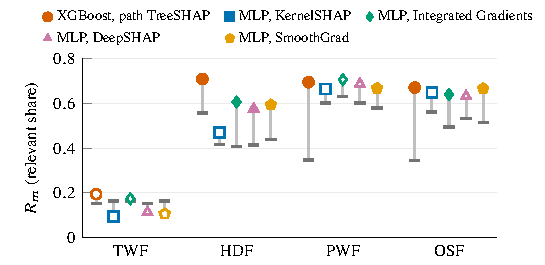
\includegraphics[width=0.7\textwidth]{figures/explainer_dependence.pdf}
\caption{Relevant share of each mechanism under XGBoost with path-dependent
TreeSHAP and an MLP with four explainers (markers; filled: aligned). Bars mark
each pipeline's own shuffled-label null mean, which is higher for the MLP on HDF, PWF, and OSF.}
\label{fig:explainers}
\end{figure}
\paragraph{Selected component checks} The ablations below concern rejection of a shuffled-label model, avoidance of an optimistic in-sample TWF pass, and detection of the strong planted shortcut at 300,000 observations. A global ranking has no statistical verdict for these checks; the table is not a general benchmark of explanation methods.

\begin{table}[htbp]
\centering
\begin{threeparttable}
\caption{Audit-component ablations on three selected diagnostic checks.}
\label{tab:compare}
\footnotesize
\setlength{\tabcolsep}{3pt}
\begin{tabular}{@{}l>{\centering\arraybackslash}b{1.25cm}>{\centering\arraybackslash}b{1.25cm}>{\centering\arraybackslash}b{1.25cm}@{}}
\toprule
Design & Rejects shuffled labels & Avoids in-sample TWF pass & Detects shortcut at $3\cdot10^5$ \\
\midrule
Global SHAP ranking & -- & -- & -- \\
Naive null & No & No & No \\
In-sample SHAP & Yes & No & No \\
Relevant share $R_m$ only & Yes & Yes & No \\
\addlinespace
\textbf{Full audit} & \textbf{Yes} & \textbf{Yes} & \textbf{Yes} \\
\bottomrule
\end{tabular}
\begin{tablenotes}[flushleft]
\footnotesize
\item ``--'': no statistical result. The naive null passes all four
mechanisms ($p=0.002$); in-sample SHAP, tested against the shuffled-label
null, passes TWF ($p=0.004$) and misses the shortcut ($p_C=0.06$).
\end{tablenotes}
\end{threeparttable}
\end{table}

\section{Several weak proxies}

Stage 24 replaces the single planted sensor by three sensors $s_{i,k}=z_{i,\mathrm{HDF}}+\epsilon_{i,k}$ with independent noise of the same $\sigma$, all outside $E_{\mathrm{HDF}}$ ($K=500$). \Cref{tab:proxies} reports their attribution and the HDF tests. Together the proxies carry more information than one sensor at the same $\sigma$, and HDF loses alignment at a larger $\sigma$ (0.4 versus 0.3). The model spreads attribution over the three proxies, so the largest single excess, which $C_m$ tests, grows slowly; the proxies' summed excess is not tested by $C_m$. The null mean of $C_{\mathrm{HDF}}$ also rises (0.04 to 0.09), because shuffled-label models also attribute to the proxies. Test F1 stays between 0.83 and 0.91, and PWF and OSF remain aligned.

\begin{table}[htbp]
\centering
\caption{Three planted proxies: summed and largest proxy share of HDF attribution, summed proxy excess, $C_{\mathrm{HDF}}$ (null mean), and Holm-adjusted $p$-values for HDF ($K=500$). Single sensor of the paper for comparison: share 0.13 at $\sigma=0.35$ (aligned) and 0.35 at $\sigma=0.25$ (flagged).}
\label{tab:proxies}
\small
\begin{tabular}{@{}lccccccl@{}}
\toprule
$\sigma$ & Sum share & Max share & Sum excess & $C_{\mathrm{HDF}}$ (null) & $p_R$ & $p_D$ / $p_C$ & Verdict \\
\midrule
1.0 & 0.07 & 0.03 & 0.00 & 0.008 (0.040) & .008 & .008 / 1.000 & aligned \\
0.67 & 0.11 & 0.05 & 0.03 & 0.027 (0.058) & .008 & .008 / 1.000 & aligned \\
0.5 & 0.17 & 0.07 & 0.09 & 0.047 (0.073) & .008 & .008 / 1.000 & aligned \\
0.4 & 0.32 & 0.13 & 0.25 & 0.108 (0.082) & .479 & .008 / .974 & not aligned \\
0.35 & 0.38 & 0.14 & 0.30 & 0.114 (0.086) & .838 & .008 / .902 & not aligned \\
0.25 & 0.54 & 0.25 & 0.46 & 0.227 (0.088) & 1.000 & .182 / .024 & flagged \\
\bottomrule
\end{tabular}
\end{table}

\section{Stability across seeds and backgrounds}

Over the primary seed and seeds 1--4, $R_m$ ranges over 0.19--0.20 (TWF), 0.70--0.72 (HDF), 0.68--0.70 (PWF), and 0.66--0.68 (OSF), $D_m$ over at most 0.04, and the three most attributed features of each mechanism are identical in all five runs (pairwise top-3 Jaccard 1.0). Over seven interventional TreeSHAP configurations (100, 500, and 1{,}000 background observations; three background seeds), $R_m$ varies by at most 0.015 and all verdicts agree. Without the engineered features, the excess of $R_m$ over its null mean falls from 0.04 to 0.02 (TWF), 0.15 to 0.06 (HDF), 0.35 to 0.25 (PWF), and 0.33 to 0.23 (OSF).

\section{Sensitivity analyses}

\paragraph{Conditional group Shapley} \Cref{tab:cond} varies the kernel bandwidth and the grouping (five groups with tool wear separated from the overstrain features). TWF is aligned in every setting; the other mechanisms lose alignment at bandwidth 0.6, where the kernel averages over most of the data, and HDF's relevant share also under the split.

\begin{table}[htbp]
\centering
\caption{Conditional group Shapley: $R_m$ (null mean) and Holm-adjusted $p_R$/$p_D$ ($K=200$); no outside-set test is significant.}
\label{tab:cond}
\small
\begin{tabular}{@{}lllll@{}}
\toprule
Setting & TWF & HDF & PWF & OSF \\
\midrule
bandwidth 0.15 & 0.59 (0.33) .020/.020 & 0.73 (0.57) .020/.020 & 0.68 (0.37) .020/.020 & 0.85 (0.60) .020/.020 \\
bandwidth 0.3 & 0.54 (0.30) .020/.020 & 0.63 (0.55) .020/.040 & 0.65 (0.42) .020/.020 & 0.80 (0.61) .020/.040 \\
bandwidth 0.6 & 0.42 (0.28) .020/.020 & 0.55 (0.51) .129/.239 & 0.47 (0.38) .104/.060 & 0.65 (0.57) .129/.239 \\
five groups, 0.3 & 0.34 (0.21) .020/.020 & 0.54 (0.48) .070/.030 & 0.61 (0.40) .020/.020 & 0.86 (0.66) .020/.030 \\
\bottomrule
\end{tabular}
\end{table}

\paragraph{CWRU defect-frequency bands} \Cref{tab:bands} varies the half-width of the defect-frequency bands and adds the third harmonic (original recordings, $K=1{,}000$).

\begin{table}[htbp]
\centering
\caption{CWRU: $R_m$ (null mean) and Holm-adjusted $p_R$/$p_D$ for each band definition; no outside-set test is significant.}
\label{tab:bands}
\small
\begin{tabular}{@{}llll@{}}
\toprule
Bands & Inner race & Ball & Outer race \\
\midrule
$\pm0.05$ orders, harmonics 1--2 & 0.45 (0.26) .012/.090 & 0.08 (0.11) .793/.098 & 0.42 (0.17) .003/.021 \\
$\pm0.15$ orders, harmonics 1--2 (paper) & 0.44 (0.23) .004/.030 & 0.13 (0.17) .773/.211 & 0.39 (0.15) .003/.027 \\
$\pm0.3$ orders, harmonics 1--2 & 0.41 (0.23) .010/.018 & 0.22 (0.12) .015/.018 & 0.36 (0.17) .003/.015 \\
$\pm0.15$ orders, harmonics 1--3 & 0.44 (0.26) .004/.009 & 0.14 (0.22) .963/.326 & 0.43 (0.17) .003/.009 \\
\bottomrule
\end{tabular}
\end{table}

\paragraph{Minimum outside-set excess} Across all stored results, the significant outside-set flags with excess at most 0.047 are the seven TWF flags on temperatures in the scaling runs, an in-sample TWF flag (0.034), and the TEP IDV5 flag (0.026); every planted sensor, the CWRU gain shortcut, and every omitted trigger has an excess of at least 0.165, and the remaining flags lie between (SmoothGrad on the MLP, 0.074; failure-only background, 0.113). A minimum excess of 0.05 separates the two groups in these data; it was chosen after seeing them and is exploratory (stage 19).

\section{TEP Temporal Models} Adding each variable's 30-minute mean and change as inputs (attribution summed per variable) raises pooled fault-active-class F1 across both fault types to 0.94 and IDV5 recall from 0.39 to 0.86. IDV4 stays aligned ($R=0.68$, null 0.07); IDV5's loop share rises to 0.54 (null 0.06), and the E-feed excess shrinks from 0.026 to 0.011 but remains significant, so IDV5 stays flagged. An LSTM (32 units, 20 epochs) on the same samples as 30-minute sequences, explained by Integrated Gradients (64 steps from the training-mean sequence) with attribution summed over time per variable, reaches pooled fault-active-class F1 0.91 across both fault types and IDV5 recall 0.81 (stage 22, $K=200$). All TEP variants use the same 400 runs and sampled endpoints, with five stratified group folds holding out complete runs (seed 42); no sequence from a held-out run enters training. For the LSTM, each variable is standardized using the training fold's mean and standard deviation over sequence time steps. The one-layer LSTM is trained with Adam (learning rate 0.003, batch size 256), binary cross-entropy, and a fixed probability threshold of 0.5. Integrated Gradients explains the logit; signed attributions are summed over the ten time steps for each variable before taking the absolute value. Each null draw permutes labels within each run and refits all five models, recomputes training-fold scaling, and re-explains the held-out observations. Mechanism groups retain their original fault-active definitions. This reference does not preserve temporal dependence in the labels and is not a temporal exchangeability guarantee. IDV4 is aligned ($R=0.43$, null 0.08), and IDV5 passes both alignment tests ($R=0.23$, null 0.06) but is flagged on the D-feed valve (excess 0.011, $p=0.010$).

\paragraph{Rotated-label null} Within each run the 32 samples are in time order, with 16 normal samples followed by 16 fault-active ones. The rotated-label null shifts each run's label sequence circularly by an offset drawn uniformly from 0--31, so the fault-active labels remain one contiguous block (wrapping around the run's end), and refits and re-explains as above ($K=200$; \texttt{15\_tep\_audit.py --null shift}). \Cref{tab:tepshift} compares it with the within-run permutation. Null means rise slightly, and every verdict is unchanged; all adjusted $p$-values remain at the minimum or 1. The LSTM was not rerun under this null.

\begin{table}[htbp]
\centering
\caption{TEP under the within-run permutation and the rotated-label null: $R_m$ (null mean) and Holm-adjusted $p_R$/$p_D$/$p_C$ ($K=200$).}
\label{tab:tepshift}
\small
\begin{tabular}{@{}llll@{}}
\toprule
Model & Null & IDV4 & IDV5 \\
\midrule
Static & permutation & 0.75 (0.07) .010/.010/1.0 & 0.22 (0.06) .010/.010/.010 \\
Static & rotation & 0.75 (0.08) .010/.010/1.0 & 0.22 (0.06) .010/.010/.010 \\
30-min features & permutation & 0.68 (0.07) .010/.010/1.0 & 0.54 (0.06) .010/.010/.010 \\
30-min features & rotation & 0.68 (0.08) .010/.010/1.0 & 0.54 (0.07) .010/.010/.010 \\
\bottomrule
\end{tabular}
\end{table}

\end{document}
